% !TeX encoding = UTF-8
% !TeX spellcheck = de_DE
% !TeX program = pdflatex


% % % % % % % % %
% offene Punkte
% % % % % % % % %

%TODO „Konzentrationshilfe für eine längere Sitzung“ → auf den Leerseiten einfügen
%TODO Auzählungszeichen (z.B römisch 1) für Abschnitt „Infoblatt zum StartPaket“ vor dem 1. Kapitel

% % % % % % % % % % % % % % % % % %
% Dokumentation und Informationen
% % % % % % % % % % % % % % % % % %

% PDFs einbinden: keine technisch schöne Lösung, aber es geht schnell.
% Verbesserung für die Zukunft: Wiki-Seiten in geeignetem Format (z.B. DocBook-XML) exportieren (evtl. sogar automatisiert) und in LaTeX parsen.

% DRUCK
%  auf A4, mit Druckrändern von ca. 7mm an den kurzen und 6mm an den langen Kanten
%   (Die über die PDFs gelegten Seitennummern und Kapitelüberschriften sehr knapp an diesem Rand.)

% pdfbook --short-edge stuve-handbuch-1.pdf
% bzw.
% pdfjam --booklet 'true' --landscape --suffix book --signature '4' --preamble '\usepackage{everyshi}
% \makeatletter
% \EveryShipout{\ifodd\c@page\pdfpageattr{/Rotate 180}\fi}
% \makeatother
% ' -- stuve-handbuch.pdf - 







% Seitennummern in PDFs einfügen, Kapitelüberschriften Rand:
%  http://stackoverflow.com/questions/1603301/how-to-add-page-numbers-to-postscript-pdf
%  http://tex.stackexchange.com/questions/48641/chapter-title-in-rotated-vertical-box-at-the-margin

% Doku zum Einbinden von PDF-Seiten mit pdfpages:
%  http://www.ctan.org/tex-archive/macros/latex/contrib/pdfpages/pdfpages.pdf

% pdfpages verwendet letzendlich \includegraphics aus graphicx
%  ab Seite 9 aus http://ctan.mackichan.com/macros/latex/required/graphics/grfguide.pdf

% Altenative, ursprüngliche Realisierung mit pdfjam:
% pdfjam --outfile ./stuve-handbuch.pdf --fitpaper 'true' --twoside --paper a4paper --no-tidy --frame 'false' --rotateoversize 'false' --suffix joined -- 00-intro.pdf - 10-infoblatt-startpaket.pdf - aa-fuellseiten.pdf 1 20-grundsaetzliches-fsr.pdf - 40-aufgabenverteilung.pdf - 55-beschlusssammung-stex.pdf -  60-vs-dossier-rechtliche-rahmenbedingungen.pdf 1-17 aa-fuellseiten.pdf 2 70-organisationssatzung.pdf - 75-finanzordnung.pdf - 91-struktur	%fitpaper=true,-uebersicht.pdf - 92-struktur-akad_selbstverw.pdf - 93-struktur-besetzung-kontrolle.pdf - 99-extro.pdf -


\documentclass[
	10pt,
	a5paper,
	twoside
	]
	{book}

% !TeX root = ../stuve-handbuch-latex.tex
% !TeX encoding = UTF-8
% !TeX spellcheck = de_DE
% !TeX program = pdflatex



% Dokument-Metadaten:
% % % % % % % % % % %

\title{StuVe-Handbuch: Gremien, Beschl\"usse und Statuten}
\date{\today}
\author{et al.\email{stuve.kontakt@uni-ulm.de}}


% Schrifen, Sprache und Co.:
% % % % % % % % % % % % % % %

\usepackage[utf8]{inputenc}
\usepackage[T1]{fontenc}					% für echte Umlaute und mehr…
\usepackage{lmodern}						% schönere Schrift, v.a in PDFs
\renewcommand{\familydefault}{\sfdefault}
\usepackage[ngerman]{babel}					% deutsche Sprachvariante (Inhaltsverzeichnis, …)
\usepackage{setspace}
\usepackage{tipa}							% für IPA Zeichen


% Textbild:
% % % % % %

\setlength{\parindent}{0pt}        %  kein Einruecken bei Absaetzen 


% „Seiteneinstellungen“:
% % % % % % % % % % % %

% Fußnoten:
\usepackage{perpage}
\MakePerPage{footnote}		%perpage package command: fußnoten

\usepackage[left=2.2cm, right=2cm, top=1cm, bottom=1cm]{geometry}
% Diese „Seitengeometrie“ passt ganz gut zu einem Heftchen aus DIN A5 Seiten mit einer Ringbindung (Plastik), wie man sie im Druckraum der StuVe herstellen kann.
% Abschätzung / Uberlegungen:
%  * Die Rinbindung wird bei 38 Blatt DIN A5 (76 Seiten mi PDF) mit 80 g/m² mit einem 10 mm Binderücken aus Plastik ganz gut.
%  * Die Löcher für die Ringbindung nehmen ca. 7 mm vom inneren Papierrand in der Breite weg.
%  * Am äußeren Rand der Seiten nehmen dir überlagerten Seitennummern und die denkrechten Abschnittsüberschriften optisch noch Platz ein. Die entsprechenden Maße finden sich unten (Definition des eigenen 'fancypagestyle'),
%  * Eigentlich ist's so gedacht, dass das Heft ohne nachträgliche Skalierung auf dem Weg zum Drucker gedruckt wird, jedoch passiert das je nach Drucker und Druckertreiber evtl. trotzdem.



\usepackage{layout}							% für \layout{} → Darstellung der aktuellen Ränder und Co.
\usepackage{totcount}						% Zählen der Gesamtzahl, z.B. von Kapiteln
\regtotcounter{chapter}

\usepackage[final]{pdfpages}
\usepackage{graphicx}


% Überschriften und Inhaltsverzeichnis formatieren:
% % % % % % % % % % % % % % % % % % % % % % % % % %

\addto\captionsngerman{\renewcommand{\chaptername}{Teil}}

\usepackage{titlesec}
\usepackage{fancyhdr}

\renewcommand*{\chaptermark}[1]{ \markboth{\thechapter: ##1}{} }%

%\titlespacing*{\chapter}{0pt}{}{20pt}
\titleformat{\chapter}[display]{\normalfont\huge\bfseries}{\flushright \chaptertitlename\ \thechapter}{5pt}{\flushright \Huge}

% Neues Kommando zum individuellen Einfügen des Inahltsverzeichnisses:
\makeatletter
\newcommand*{\toccontents}{\@starttoc{toc}}
\makeatother

\usepackage{titletoc}

% Merkhilfe:
% \titlecontents{⟨Abschnitt⟩}[⟨Links⟩]{⟨Gesamtformatierung⟩}{⟨Vor dem Label⟩}{⟨Nach dem Label⟩}{⟨Abstandsfüller & Seitenzahl⟩}[⟨Rechts⟩]
\titlecontents{chapter}[1.5em]{\small}{\contentslabel{1em}}{}{\titlerule*[0.3pc]{.}\contentspage}
\titlecontents{section}[2.5em]{\footnotesize}{\contentslabel{1em}}{}{\titlerule*[0.3pc].{}\contentspage}
%\titlecontents{subsection}[6.7em]{}{\contentslabel{2.95em}}{}{\titlerule*[0.3pc]{.}\contentspage} 
%\titlecontents{subsubsection}[10.6em]{}{\contentslabel{3.8em}}{}{\titlerule*[0.3pc]{.}\contentspage}
%\titlecontents{paragraph}[15.25em]{}{\contentslabel{4.6em}}{}{\titlerule*[0.3pc]{.}\contentspage}


% Abschnittsmarkierungen (äußerer Seitenrand)
% % % % % % % % % % % % % % % % % % % % % % %

\usepackage{tikz}
\usepackage{color}
\usetikzlibrary{shapes.misc}
\usetikzlibrary{calc}
\usetikzlibrary{positioning}
\usepackage{lipsum}

\usepackage{etoolbox}
% Patch the sectioning commands to provide a hook to be used later
\preto{\chapter}{\def\leveltitle{\chaptertitle}}
\preto{\section}{\def\leveltitle{\sectiontitle}}
\preto{\subsection}{\def\leveltitle{\subsectiontitle}}
\preto{\subsubsection}{\def\leveltitle{\subsubsectiontitle}}

\makeatletter
% \@sect is called with normal sectioning commands
% Argument #8 to \@sect is the title
% Thus \section{Title} will do \gdef\sectiontitle{Title}
\pretocmd{\@sect}
{\expandafter\gdef\leveltitle{#8}}
{}{}
% \@ssect is called with *-sectioning commands
% Argument #5 to \@ssect is the title
\pretocmd{\@ssect}
{\expandafter\gdef\leveltitle{#5}}
{}{}
% \@chapter is called by \chapter (without *)
% Argument #2 to \@chapter is the title
\pretocmd{\@chapter}
{\expandafter\gdef\leveltitle{#2}}
{}{}
% \@schapter is called with \chapter*
% Argument #1 to \@schapter is the title
\pretocmd{\@schapter}
{\expandafter\gdef\leveltitle{#1}}
{}{}
\makeatother

%\newcommand\MyColor{
%	\ifcase\thechapter blue!30\or red!30\or olive!30\or magenta!30\else yellow!30\fi} 
\newcommand\MyColor{ black!30 }

\fancypagestyle{plain}{%
	%% Clear all headers and footers
	\fancyhf{}
	%% Right headers on odd pages
	\fancyhead[RO]{%
			\begin{tikzpicture}[overlay,remember picture]
			\ifdefined\chaptertitle
			\node[
				fill=\MyColor, text=black,
				font=\footnotesize,
				inner ysep=4pt, inner xsep=4pt,
				rounded rectangle,
				anchor = west,
				%xshift=-0mm,
				%yshift=-0mm,
				%text width=3cm,
				text height=0.3cm,
				rotate=90
			]
			% 21 cm an der kurzen Kante der A4 bzw. langen Kante der A5 Seite:
			%   21 cm - 6 mm Druckrand oben - 6 mm Druckrand unten - 6 mm Länge Bobbel Seitenzahl = 19,2 cm
			at ($ (current page.north east) + (-0.9cm, -0.7cm) + (-0.15cm, -0.3cm) + (0cm, -19.3 / \totvalue{chapter} * \thechapter cm) $)
			{\sffamily\normalsize\nouppercase{\thechapter: \chaptertitle}};
%			{\sffamily\normalsize\nouppercase{\thechapter: }};
			\fi
			\node[
				fill=\MyColor,text=black,
				font=\footnotesize,
				inner ysep=4pt, inner xsep=4pt,
				rounded rectangle,
				%anchor = north east,
				%xshift=-0mm,
				%yshift=-0mm,
				%text width=5cm,
				text height=0.3cm,
				rotate=0
			]
			at ($ (current page.north east) + (-0.9cm, -0.7cm) + (-0.15cm, -0.15cm) $)
			{\sffamily\normalsize\nouppercase{\thepage}};
			\end{tikzpicture}
	}
	%% Left headers on even pages
	\fancyhead[LE]{%
			\begin{tikzpicture}[overlay,remember picture]
			\ifdefined\chaptertitle
			\node[
			fill=\MyColor,text=black,
			font=\footnotesize,
			inner ysep=4pt, inner xsep=4pt,
			rounded rectangle,
			anchor=east,
			%xshift=-0mm,
			%yshift=-0mm,
			%text width=3cm,
			text height=0.3cm,
			rotate=270
			]
			at ($ (current page.north west) + (0.9cm, -0.7cm) + (0.15cm, -0.3cm) + (0cm, -19.3 / \totvalue{chapter} * \thechapter cm) $)
			{\sffamily\normalsize\nouppercase{\thechapter: \chaptertitle}};
%			{\sffamily\normalsize\nouppercase{\thechapter:}};
			\fi
			\node[
			fill=\MyColor,text=black,
			font=\footnotesize,
			inner ysep=4pt, inner xsep=4pt,
			rounded rectangle,
			%anchor= ,
			%xshift=-0mm,
			%yshift=-0mm,
			%text width=5cm,
			text height=0.3cm,
			rotate=0
			]
			at ($ (current page.north west) + (0.9cm, -0.7cm) + (0.15cm, -0.15cm) $)
			{\sffamily\normalsize\nouppercase{\thepage} };
			\end{tikzpicture}
	}
	\renewcommand{\headrulewidth}{0pt}
	\renewcommand{\footrulewidth}{0pt}
	%\fancyfoot[R]{\thepage}
}
% ----------------------------------------------------------------



% Hyperref-Paket (muss immer als letztes geladen werden)
% % % % % % % % % % % % % % % % % % % % % % % % % % % % %

\usepackage{hyperref}

\hypersetup{
	pdftitle=StuVe-Handbuch,
	pdfauthor=et. al.,
	pdfsubject={Handbuch},
	pdfproducer={pdflatex},
	%	colorlinks=false,
	pdfborder=0 0 0	% keine Box um die Links!
}


% Eigene Kommandos:
% % % % % % % % % %

% Führende Null für's Datum:
\newcommand{\leadingzero}[1]{\ifnum #1<10 0\the#1\else\the#1\fi} 

\begin{document}

%\layout{}

\frontmatter

\pagestyle{plain}		% Standardseitenlayout
\footnotesize			% Standardschriftgröße

% !TeX root = ../stuve-handbuch-latex.tex
% !TeX encoding = UTF-8
% !TeX spellcheck = de_DE
% !TeX program = pdflatex

{
\newgeometry{left=2.7cm, right=2cm, top=1cm, bottom=1cm}
\pagestyle{empty}

%----------------------------------------------------------------------
%
%        Titelblatt
%
%----------------------------------------------------------------------

\begin{titlepage}

\null
\vfill

\begin{center}
	\vspace{2em}
	{\Huge \bfseries StuVe-Handbuch\\}
	\vspace{4em}
\end{center}

\begin{figure}[tbph]
\centering

\includegraphics[trim = 600px 0 600px 0, width = \linewidth]{./grafiken/VS_Scrabble-mod.jpg}
\end{figure}

\null
\vfill

\begin{center}
	\begin{minipage}{\textwidth}
	\begin{minipage}[b][2cm]{0.79\textwidth}
		\begin{flushleft}
			Version \the\year"~\leadingzero{\month}"~\leadingzero{\day}\\
			\vspace{0.5\baselineskip}
			StuVe / Verfasste Studierendenschaft\\
			Universität Ulm
		\end{flushleft}
	\end{minipage}
	\begin{minipage}[b][2cm]{0.2\textwidth}
		\begin{flushright}
			
\includegraphics[height=1.6cm]{./grafiken/stuve_logo_gedreht-leicht_grau.png}
		\end{flushright}
	\end{minipage}
\end{minipage}
\end{center}

\end{titlepage}

%\restoregeometry
%}

%----------------------------------------------------------------------
%
%        Innenseite
%
%----------------------------------------------------------------------
%{
%\newgeometry{left=2.7cm, right=2cm, top=1cm, bottom=1cm}

\newpage
\footnotesize
\bigskip


\begin{center}

\null
\vspace{2em}
\textbf{Wichtige Adressen}

\bigskip
Homepage\\
\textit{http://www.uni-ulm.de/stuve}

\bigskip
Wiki\\
\textit{https://wiki.asta.uni-ulm.de}

\bigskip
E-Mail\\
\textit{stuve@uni-ulm.de\\
stuve.exekutive@uni-ulm.de\\
stuve.kontakt@uni-ulm.de}\\

\null
\begin{minipage}{0.5\textwidth}
	\scriptsize
	\begin{center}
	Für Organisatorisches oder falls es wichtige Gründe gibt die StuVe-Liste nicht zu nutzen gibt es für StuPa und FSR eigene Listen. \\\textbf{Grundsätzlich soll jedoch stuve@uni-ulm.de genutzt werden!}
	\end{center}
\end{minipage}

\null
\textit{stuve.parlament@uni-ulm.de\\
stuve.fachschaftenrat@uni-ulm.de}

\bigskip
Mailinglisten\\
{\scriptsize (An- und Abmelden, Empfangsmodus, ...)}\\
\textit{https://imap.uni-ulm.de/lists}

\null
\vfill
\begin{minipage}{0.8\textwidth}
\footnotesize Dieses Heft gehört:~\hrulefill~;-)
\end{minipage}
\vspace{2em}
\null

\end{center}

\restoregeometry
}


\setcounter{page}{1}

% !TeX root = ../stuve-handbuch-latex.tex
% !TeX encoding = UTF-8
% !TeX spellcheck = de_DE
% !TeX program = pdflatex


\textit{Definition: Die Verfasste Studierendenschaft der Universität Ulm (VS) setzt sich aus allen eingeschriebenen Studierenden zusammen.
Die VS bzw. die Studierenden organisieren sich in der StuVe (StudierendenVertretung)\footnote{\today: Diese Definition der StuVe fehlt noch in der Organisationssatzung, sollte demnächst ergänzt werden.}.
D.h.\ alle Organe, Strukturen und auch sonst irgendwie offiziell aktiven Studierenden bilden die „organisierte“ StuVe – im Ggs. zur gesamten Studierendenschaft.}


\section*{Zu diesem Heft}

%\vspace{1em}
%\textbf{Zu diesem Handbuch}
%\vspace{0.3em}

Für alle in der StuVe Aktiven und insbesondere die Mitglieder der StuVe-Gremien sind die hier die wichtigsten Texte zusammengefasst, die die Grundlage für die Organisation und Arbeit der StuVe bilden. Ergänzend zu diesem Handbuch soll demnächst noch ein zweites Handbuch mit Hilfen für's operative Tagesgeschäft verfügbar sein.
Es handelt sich hier nicht um ein am Stück geschriebenes Werk, sondern fast ausschließlich um eine Zusammenstellung verschiedener Texte.
Einerseits sind einfache Hilfestellungen, wie z.B.\ die Infoblätter oder Grafiken, andererseits aber auch für alle Studierenden und insbesondere die gewählten Vertreter und Aktiven rechtlich verbindliche Texte, wie z.B.\ die Organisationssatzung oder die Finanzordnung, enthalten.

Da sich die Dokumente bisweilen ändern wird auch dieses Heft immer wieder aktualisiert werden, zum Vergleich verschiedener Ausgaben dient das Datum auf der Titelseite.
Manche der enthaltenen Dokumente haben eine eigene Seitennummerierung – im gesamten Heft ist jedoch jeweils am äußeren Rand die Bezeichnungen des aktuellen Teils und eine durchgehende Seitennummern grau hinterlegt abgedruckt. Auf diese bezieht sich das folgende Inhaltsverzeichnis.


\subsection*{Inhalt}

%\vspace{1em}
%\textbf{Inhalt}
%\vspace{0.3em}

\toccontents


\subsubsection*{Nicht enthalten}
%\vspace{0.5em}
%\textbf{Nicht enthalten}
%\vspace{0.3em}
\begin{itemize}
	\item Wahlordnung
	\item Landeshoschulgesetz Baden-Württemberg (LHG)\\Informationen hierzu jedoch in Rechtliche Grundlagen und Rahmenbedingungen für die neue Studierendenvertretung.
\end{itemize}



% % % % % % % % % % % % %
%
% AB HIER PDFs EINBINDEN
%
% % % % % % % % % % % % %


% Optionen für alle einzubindenden PDFs
\includepdfset{
	pages= - ,								% standardmäßig alle Seiten eines PDFs einbinden
	pagecommand=\thispagestyle{plain},
	%openright,								% lieber lassen :P
	%frame=true,							% für den Entwurfsmodus, vor dem Druck deaktivieren
	offset = 0.2cm 0,						% Zugabe für's Binden !!! weitere offsets unten sind zusätzlich
	trim = 1cm 0cm 1cm 0cm,
}

% die einzelnen PDFs beschneiden:
%	trim = l u r o
%		→ links, unten, rechts, oben etwas abschneiden, muss leider pro PDF definiert werden.

% beschnittene PDFs werden mit dem folgenden pauschal skaliert, so dass sie die Seite gut Ausnutzen
% nur eine Dimension (height) angegeben -> für PDFs gilt keepaspectratio, bei Grafiken einzeln drauf achten
\let\ORIincludegraphics\includegraphics
\renewcommand{\includegraphics}[2][]{\ORIincludegraphics[height=0.90\paperheight,#1]{#2}}


\clearpage


\addcontentsline{toc}{chapter}{Infoblatt zum StartPaket\newline{\scriptsize\textit{\null\hspace{2em}Anleitung zum Kennenlernen wichtiger Einrichtungen und Arbeitsmaterialien}}}

\clearpage
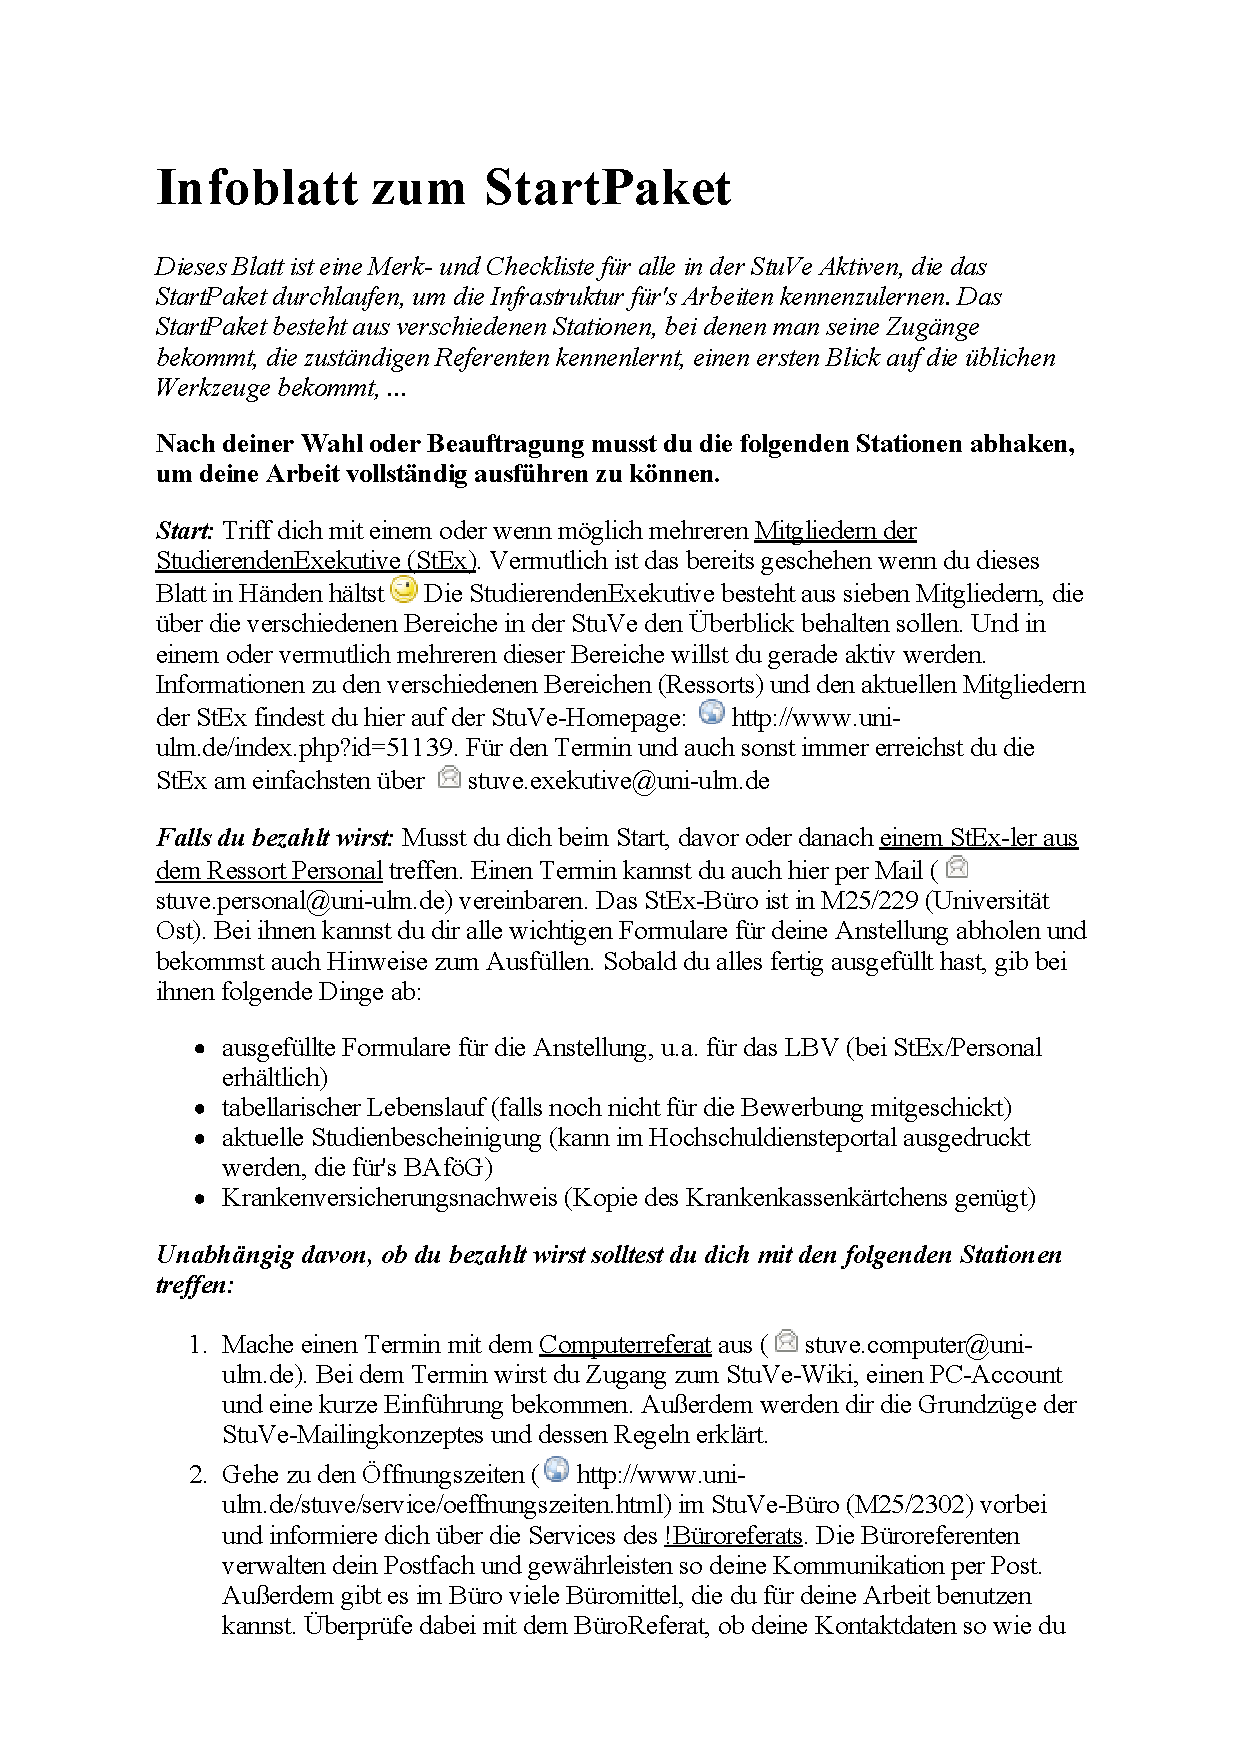
\includepdf
	[
		trim = 2cm 1.3cm 2cm 0.8cm,
	]
	{./teile/10-infoblatt-startpaket.pdf}


\mainmatter

\chapter{Gremienarbeit}
%\addcontentsline{toc}{chapter}{Gremienarbeit}

\clearpage

\addcontentsline{toc}{section}{Sitzungsfahrplan StuPa}

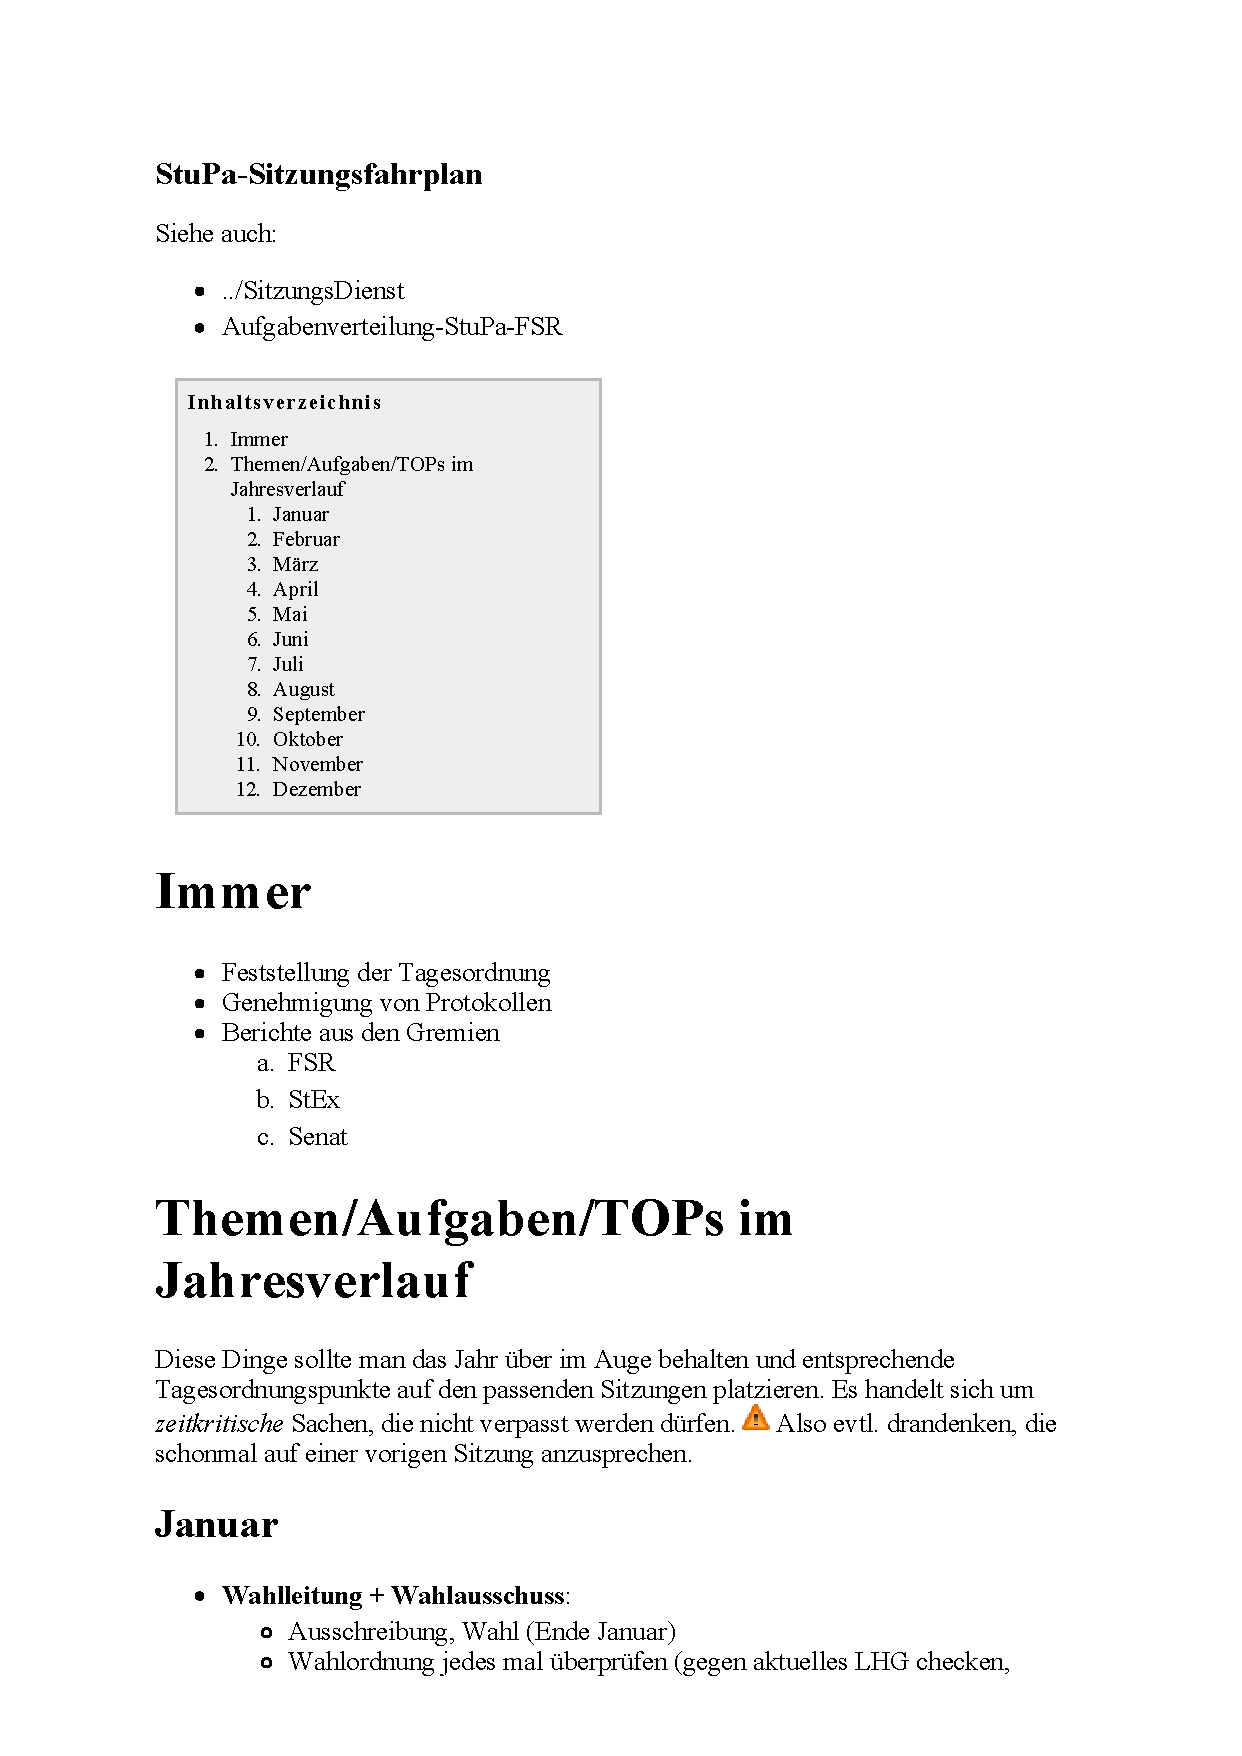
\includepdf
[
trim = 2cm 1.3cm 2cm 0.8cm
]
{./teile/40-sitzungsfahrplan-stupa.pdf}



\addcontentsline{toc}{section}{Aufgabenverteilung zwischen StuPa und FSR}

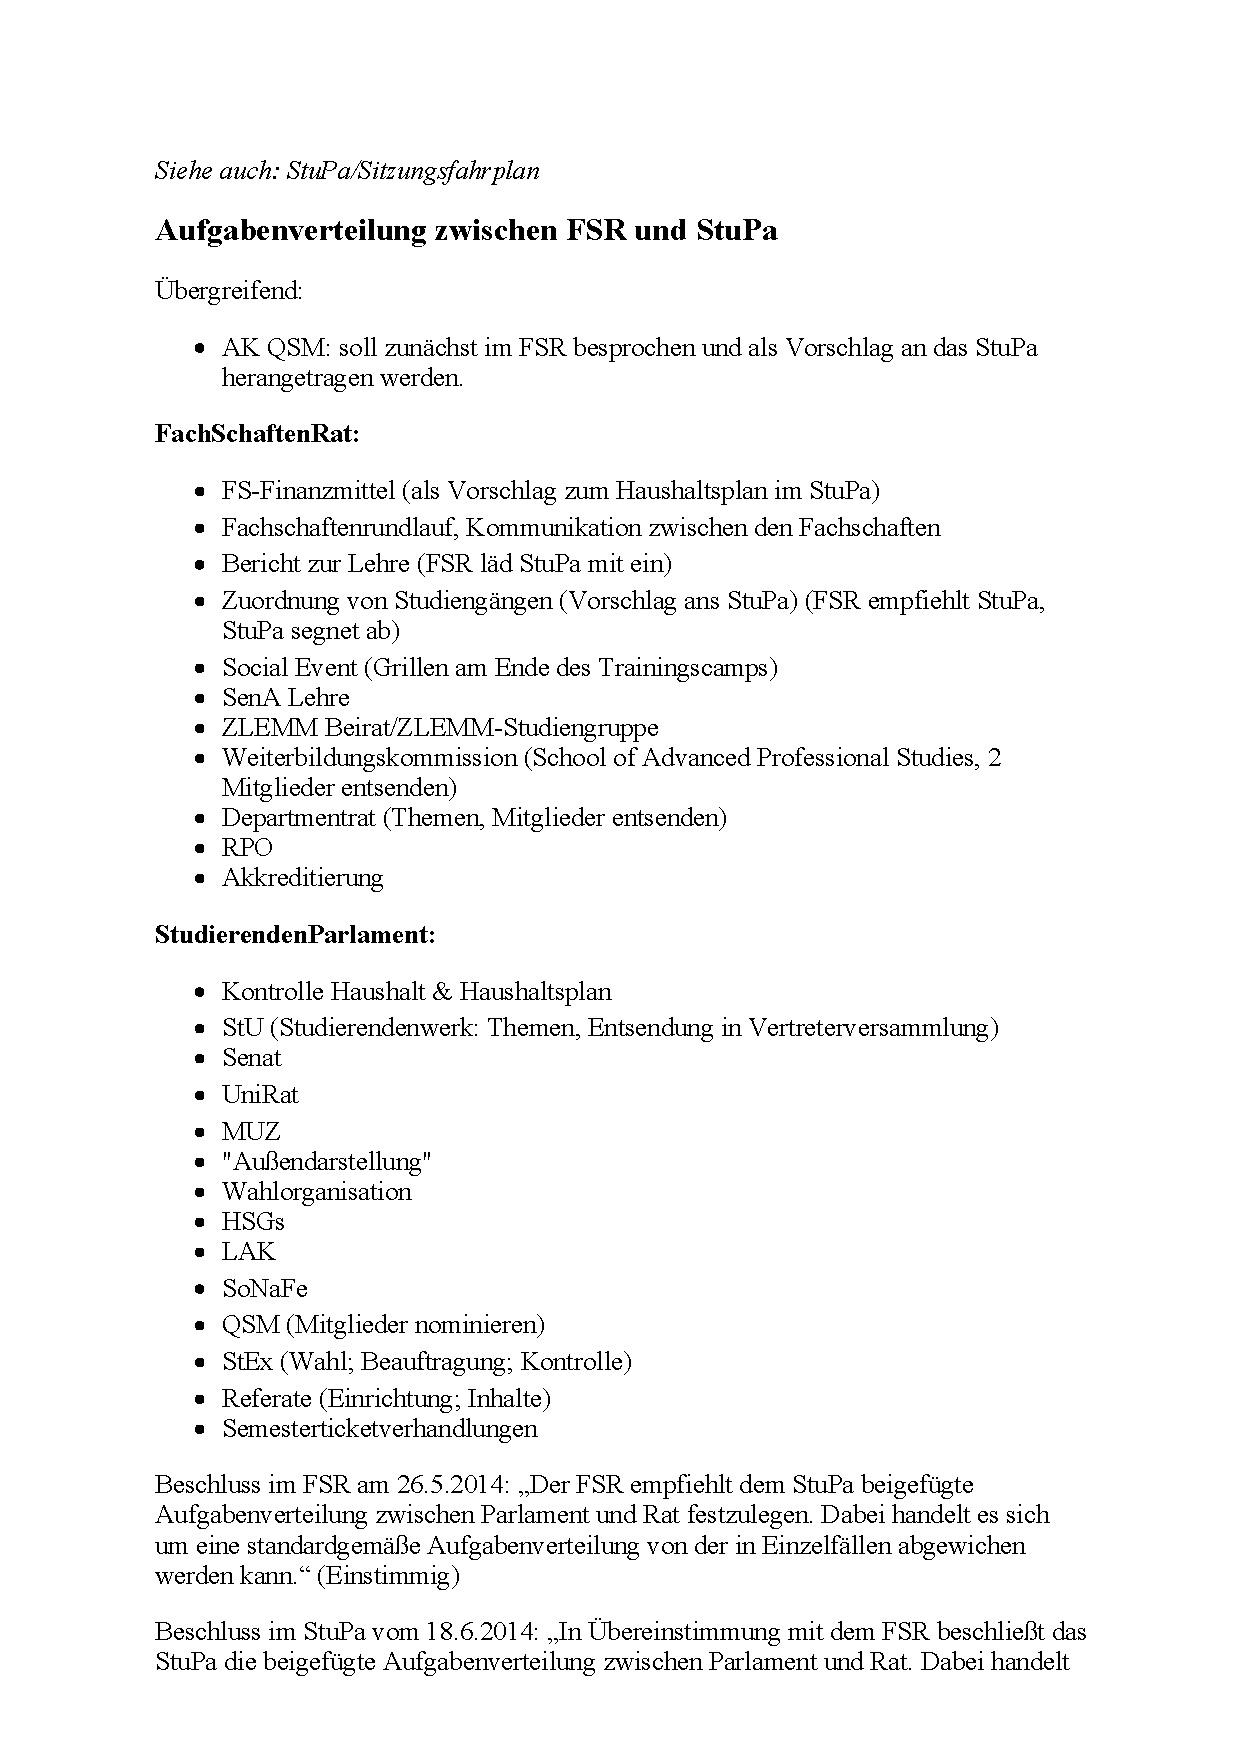
\includepdf
[
trim = 2cm 1.3cm 2cm 0.8cm
]
{./teile/40-aufgabenverteilung.pdf}

\section{Kurzbeschreibung der Arbeit und Aufgaben von StuPa, FSR und StEx}

Ergänzend zur Liste \textit{Aufgabenverteilung zwischen StuPa und FSR} hier noch die Texte zu den Gremien von der Aufgabenbeschreibung auf der Hompage\footnote{\url{http://www.uni-ulm.de/index.php?id=58311} bzw. \url{http://www.uni-ulm.de/index.php?id=51139}}.

Die Mitglieder des Studierendenparlaments und Fachschaftenrats werden in jedem Sommersemester von allen ca. 10.000 Studierenden direkt gewählt (meist im Juni).

Um dich zur Wahl für diese beiden obersten Gremien der StudierendenVertretung zu stellen, solltest du einen Wahlvorschlag einreichen (die Frist dafür ist meist im Mai). Für einen Wahlvorschlag organisierst du dich am besten mit gleichgesinnten Komilitonen unter einer gemeinsamen Überschrift und für die Themen, mit denen ihr die Wahl gewinnen wollt. Mögliche Themen gibt es viele: die Listen kommen manchmal ganz lose zu einem aktuellen Thema oder vor einem gemeinsamen kulturellen Hintergrund zusammen oder bestehen bereits jahrelang, z.B. in Anlehnung an eine der großen politischen Parteien oder die Listen beziehen sich auf eine aktuelle Bewegung.


\subsection{Studierendenparlement (StuPa)}

Das StuPa ist deine Plattform um über Themen, zu diskutieren, die die Uni Ulm wirklich bewegen. Und wenn DU dabei bist, dann bringst du DEINE Themen mit. Hier kannst du deine tollen Ideen oder auch deine Unzufriedenheit in Konstruktivität verwandeln. Zum einen hat im StuPa ein jeder Studi Rede und Atragsrecht. Also kannst du dich jederzeit einbringen, komm einfach zu einer der Sitzungen  oder besser noch kündige dein Thema vorher an! Und zum anderern kannst du dich bei den Wahlen in jedem Sommersemester wählen lassen und mitentscheiden!

Im StuPa sitzen 10 direkt gewählte parlamentarische Vertreter*innen, die sich in Listen zur Wahl aufstellen, das StuPa ist also quasi der Bundestag der Studierenden der Uni Ulm. 

Es geht um eine Vielfalt an Themen, die uns im studentischen Leben beschäftigen sollten. Wie können mehr Lernplätze in der Uni entstehen? Wieso gibt es so wenig günstigen studentischen Wohnraum? Wie geht es weiter mit dem musischen Zentrum? Wie soll an der Uni geworben werden und wie bitte lieber nicht? Und ganz grundsätzlich: Was stellt die Verfasste Studierendenschaft mit den 19 EUR Beitrag an, die sie von jedem*r Studierenden bekommt?

Du kannst dich einsetzen für Nachhaltigkeit, für soziale Themen, für Kultur und Bildung, für eine bessere Lehre oder gegen den Ulmer Leise e.V.!

Such dir Mitstreiter*innen und gründe deine Interessengruppe und tritt mit deiner „Liste“ im Juni für das StuPa-Wahlen an (Vorsicht! Die Listen müssen meist schon im Mai eingereicht werden. Mehr Informationen zur Wahl auf den Seiten des Wahlausschusses.)

Parlamentarier*in sein heißt:

\begin{itemize}
	\item Du diskutierst alle 2 Wochen auf einer StuPa-Sitzung als eine*r von 10 direkt gewählten Vertreter*innen mit.
	\item Du hast Lust an Diskussionen und bringst das nötige Durchhaltevermögen mit.
	\item Du nimmst dein Mitbestimmungsrecht wahr und sagst deine Meinung – zu den für dich im studentischen Leben relevante Themen und als Vertreter deiner 10.000 Kommilitonen.
	\item Du suchst dir den ein oder anderen Arbeitskreis aus, um das Thema, das dich am meisten packt auch konkret und außerhalb der Palamentssitzung zu betreiben. Oder du gründest ganz einfach deinen eigenen Arbeitskreis.
	\item Du trainierst deine Soft-Skills rund ums Kommunizieren und Organisieren, direkt in den Debatten und Arbeitskreisen oder in den „modernen Medien“ und sortierst endlich mal deine Mails ;-)
\end{itemize}

Einfach eine Liste von Kandidaten aufstellen und wählen lassen!



\subsection{FSR}

Der Fachschaftenrat (FSR) – das sind 24 Studierende, die jedes Jahr im Sommer von allen Studierenden gewählt werden, aus jeder der vier Fakultäten kommen sechs Vertreter*innen.

Im FSR…

\begin{itemize}
	\item ... kannst du dich in dem für uns Studierende wichtigsten Thema einbringen: der Lehre.
	\item ... darfst du auch mal im StudierendenParlament (StuPa) mitreden und dort über aktuelle allgemeine studentische Themen diskutieren und mitentscheiden.
	\item ... erlebst du hautnah, wie sich Dinge an der Uni verändern lassen und das Studieren verbessert werden kann.
	\item ... kannst du dich mit Leuten aus anderen Fachbereichsvertretungen austauschen und lernst andere engagierte Studierende kennen.
	\item ... bekommst du einen Einblick in die Organisation der StuVe.
\end{itemize}

Der Fokus des FSR liegt ganz klar auf dem Thema Lehre an der Uni. Die Mitglieder besprechen z.B. mit dem Vizepräsidenten den Bericht zur Lehre, der jährlich erstellt wird und setzen uns mit neuen Prüfungsordnungen auseinander. Wechselnde Vertreter*innen des FSR sitzen auch alle zwei Wochen im StuPa, um dort mitzudiskutieren.

Im FSR kriegst du mit was in den anderen Fachbereichen gerade so los ist und kannst dir Tipps und Anregungen von den anderen Mitgliedern holen, was deine eigene „Fachschaftsarbeit“ betrifft.

Egal ob du frisch an der Uni oder in der StuVe bist und dir das nur mal anschauen möchtest, oder ob du ein alter Hase bist, der schon genau weiß was verändert werden soll, schau doch mal bei uns vorbei! Den Termin unserer nächsten Sitzung findest hier auf der Homepage.

Haben wir dein Interesse geweckt? Dann lass dich im Juni in den FSR wählen. Und wenns dazu nicht ganz reicht, dann solltest du den deiner Meinung nach besten Vertreter*innen deine Stimme geben. Geh wählen – Denn eine starke Studierendenschaft braucht deinen Rückhalt!
Meist stellt deine FS, also die „Fachschaft“ (oder offiziell Fachbereichsvertretung), eine Kandidatenliste zur Wahl auf. Aber natürlich hat ganz einfach jeder Studi das Recht Wahlvorschläge zu organisieren, egal ob er sich nun schon in der aktiven FS einbringt oder nicht!


\subsection{StEx}

\begin{itemize}
	\item Für die Teamarbeit und die Entscheidungen ist's wichtig, dass sich alle 7 Mitglieder in der Vorlesungszeit auf einen gemeinsamen Termin für ein wöchentliches Treffen einigen können, der dauert meist eineinhalb, manchmal auch drei Stunden. Wenn man zwischendurch mal nicht kann ist das OK, aber die bisherigen Teammitglieder haben dafür auch schon ihre eigenen Stundenpläne umstellen müssen.
	\item Neben dem „Job“ mit recht konkreten Aufgaben (Finanzen kontrollieren, neuen Leuten Abläufe erklären, Ansprechpartner sein, weiterhelfen, Schreiben verfassen) ist v.a. auch echtes Engagement gefragt, weil die StEx oft die Interessen aller Studierenden vertritt, z.B. bei der Unileitung oder der Landesregierung. Das ist dann kein Bürojob zwischen neun und fünf und fordert oft besonderen Einsatz, oft auch zeitlich.
	\item Vielseitigkeit ist wichtig. Zwar wird man sein eigenes „Spezialgebiet“ haben, aber oft kommt unerwartes auf, bei dem niemand Expertise hat und am Anfang ist eine Lösung meist nicht mal in Sicht – dann muss man kreativ sein, sich informieren und Lösungen konmzipieren und mit den anderen diskutieren und entscheiden.
\end{itemize}

\textit{TODO fertig machen!}

\addcontentsline{toc}{section}{Grundsätzliches für die Arbeit im FSR \newline{\scriptsize\textit{\null\hspace{2em}für die Arbeit im FSR bewährte “best practices”}}}

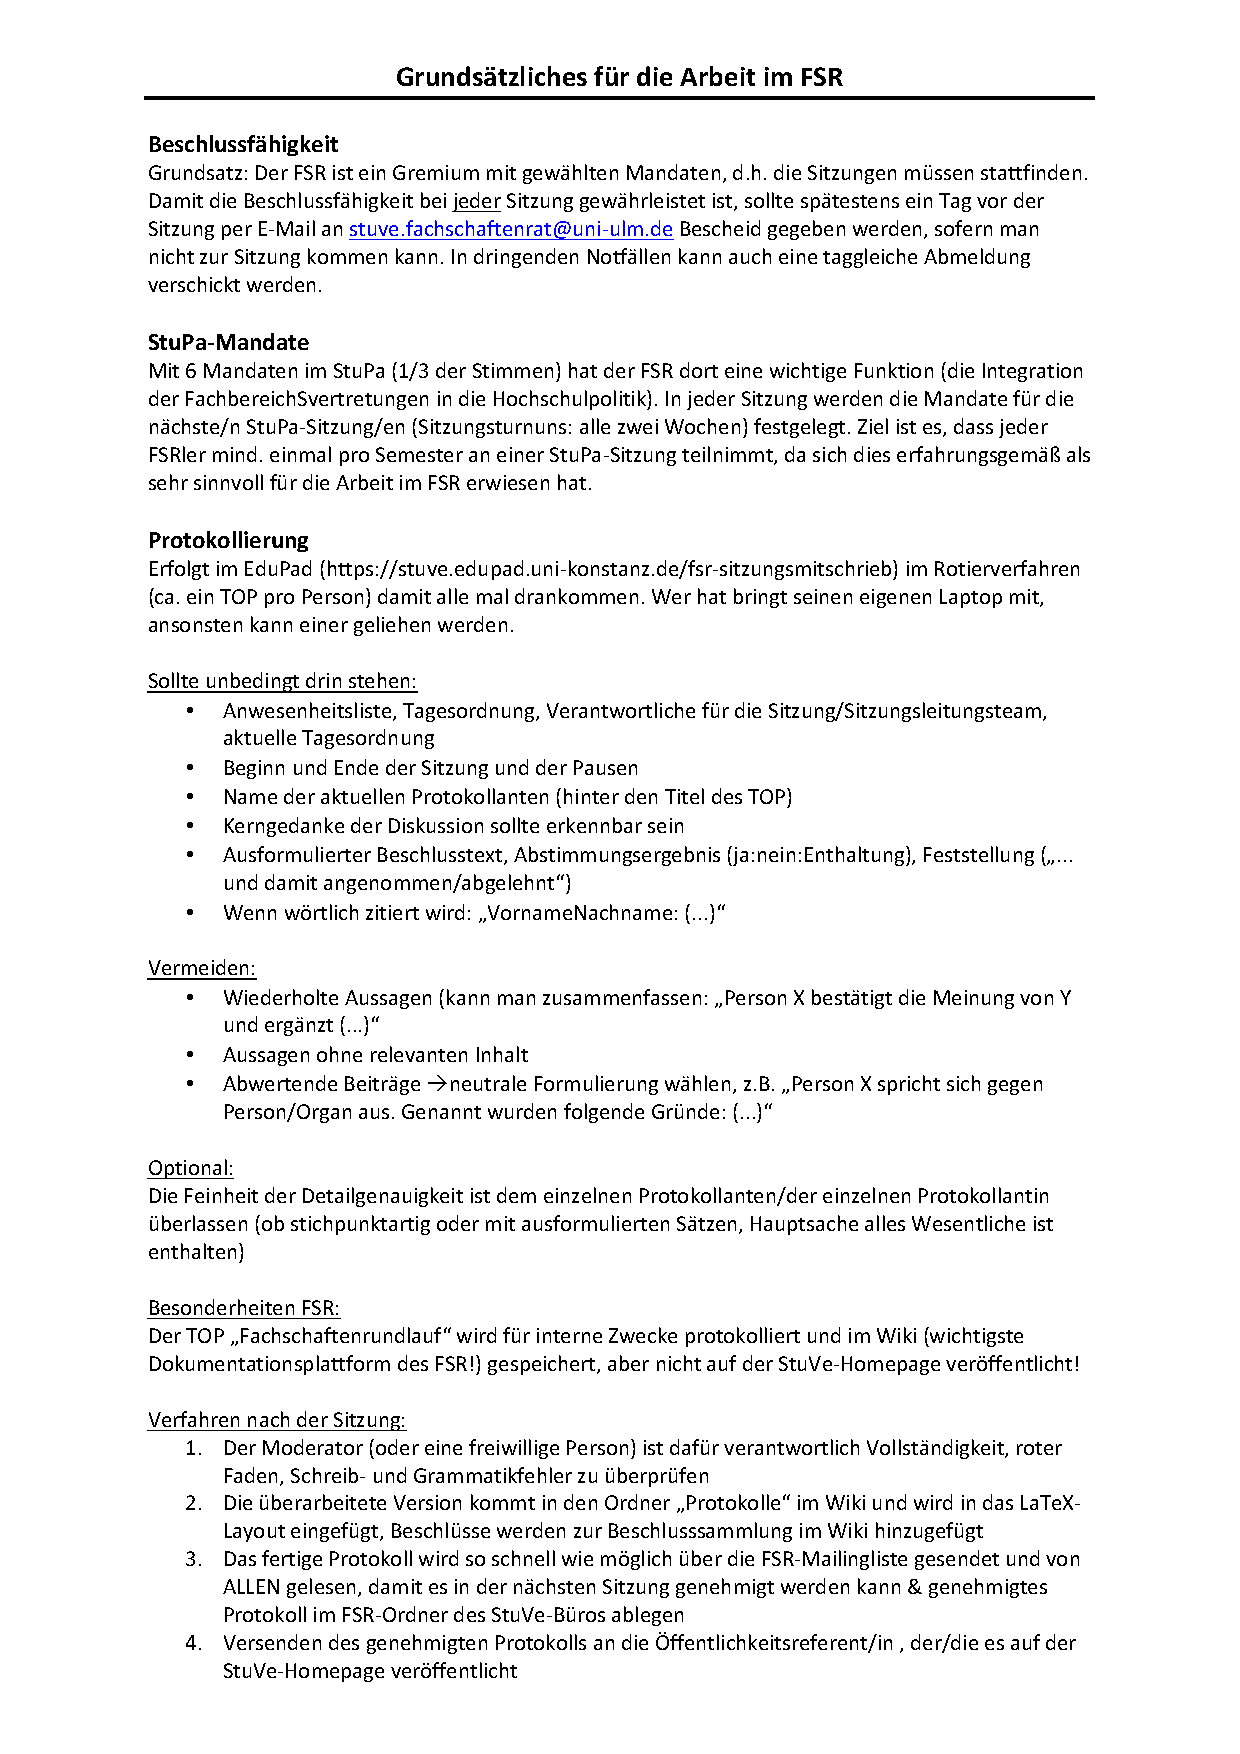
\includepdf
	[
		trim = 2cm 1cm 2cm 1cm,
		height = 0.95\paperheight,
		offset = -0.2cm 0cm
	]
	{./teile/20-grundsaetzliches-fsr.pdf}


\addcontentsline{toc}{section}{Grundsätzliches für die Arbeit im StuPa\newline{\scriptsize\textit{\null\hspace{2em}für die Arbeit im StuPa bewährte “best practices”}}}
\section*{Grundsätzliches für die Arbeit im StuPa}

\textit{Für die Arbeit im StuPa bewährte “best practices”: \textbf{TODO}.}

\clearpage



\chapter{Die ganze StuVe}

\clearpage

\section{Kommunikation}

TODO:

Erklärung der Medien: Mail, Protokolle, Homepage, Wiki, Pad, StuVe-Cloud;

lang-, mittel- und kurzfristig Dokumentation und warum die Differenzierung wichtig ist;

Motivation für die aktuelle Arbeit und die nachfolgenden Generationen etc.


\clearpage
\section{Referate}

TODO Liste der Referate und deren Mailadressen.

\cleardoublepage


\chapter{Beschlusssammlungen}


\textit{Zum Zeitpunkt des Drucks dieser Version waren die Beschlusssammlungen nicht gerade auf dem neuesten Stand (außer die des StuPa). Deshalb sind die Beschlusssammlungen in dieser Ausgabe nicht enthalten, sondern nur im Wiki zu finden.}



%\clearpage

%\addcontentsline{toc}{chapter}{Beschlusssammlungen}

%\addcontentsline{toc}{chapter}{Beschlüsse des StuPa}
%
%\addcontentsline{toc}{chapter}{Beschlüsse des FSR}
%
%\addcontentsline{toc}{chapter}{Beschlüsse der StEx}

%\includepdf
%	[
%		trim = 2cm 1.3cm 2cm 0.8cm
%	]
%	{./teile/51-beschlusssammlung-stupa.pdf}
%
%\includepdf
%[
%trim = 2cm 1.3cm 2cm 0.8cm
%]
%{./teile/53-beschlusssammlung-fsr-2.pdf}
%
%\includepdf
%[
%trim = 2cm 1.3cm 2cm 0.8cm
%]
%{./teile/53-beschlusssammlung-fsr-1.pdf}
%
%\includepdf
%	[
%		trim = 2cm 1.3cm 2cm 0.8cm
%	]
%	{./teile/55-beschlusssammlung-stex.pdf}


\chapter{Organisationssatzung}

\textit{Obacht: Anhang A der Organisationssatzung ist nicht mehr aktuell. Masterstudiengang Software Engineering (neu) und Masterstudiengang Cognitive Systems (neu) sind der FS Informatik zugeordnet; Masterstudiengang Energy Science and Technology (bisher FS Elektrotechnik) ist der FS Chemie zugeordnet.}

\clearpage


\includepdf
	[
		trim = 2cm 2cm 2cm 1cm
	]
	{./teile/70-organisationssatzung.pdf}


\chapter{Beitragsordnung, Finanzordnung}


\clearpage


\includepdf
[
trim = 2cm 2cm 2cm 1cm
]
{./teile/74-beitragsordnung.pdf}


\includepdf
	[
		trim = 2cm 2cm 2cm 1cm
	]
	{./teile/75-finanzordnung.pdf}


\chapter{Geschäftsordnung StuPa}

\clearpage


\includepdf
[
trim = 2cm 2cm 2cm 1cm
]
{./teile/77-geschaeftsordnung-stupa.pdf}



\chapter{Rechtliche Grundlagen}

\textit{Dieser Teil hat wurde zuletzt Anfang 2015 aktualisiert, allerdings wurden die Änderungen der LHG-Novelle vom April 2014 noch nicht vollständig eingearbeitet. Dieser Teil wird evtl. erst nach Lesen der Organisationssatzung klar, kann aber auch vorab schon den „großen Rahmen“ erläutern.}

\clearpage

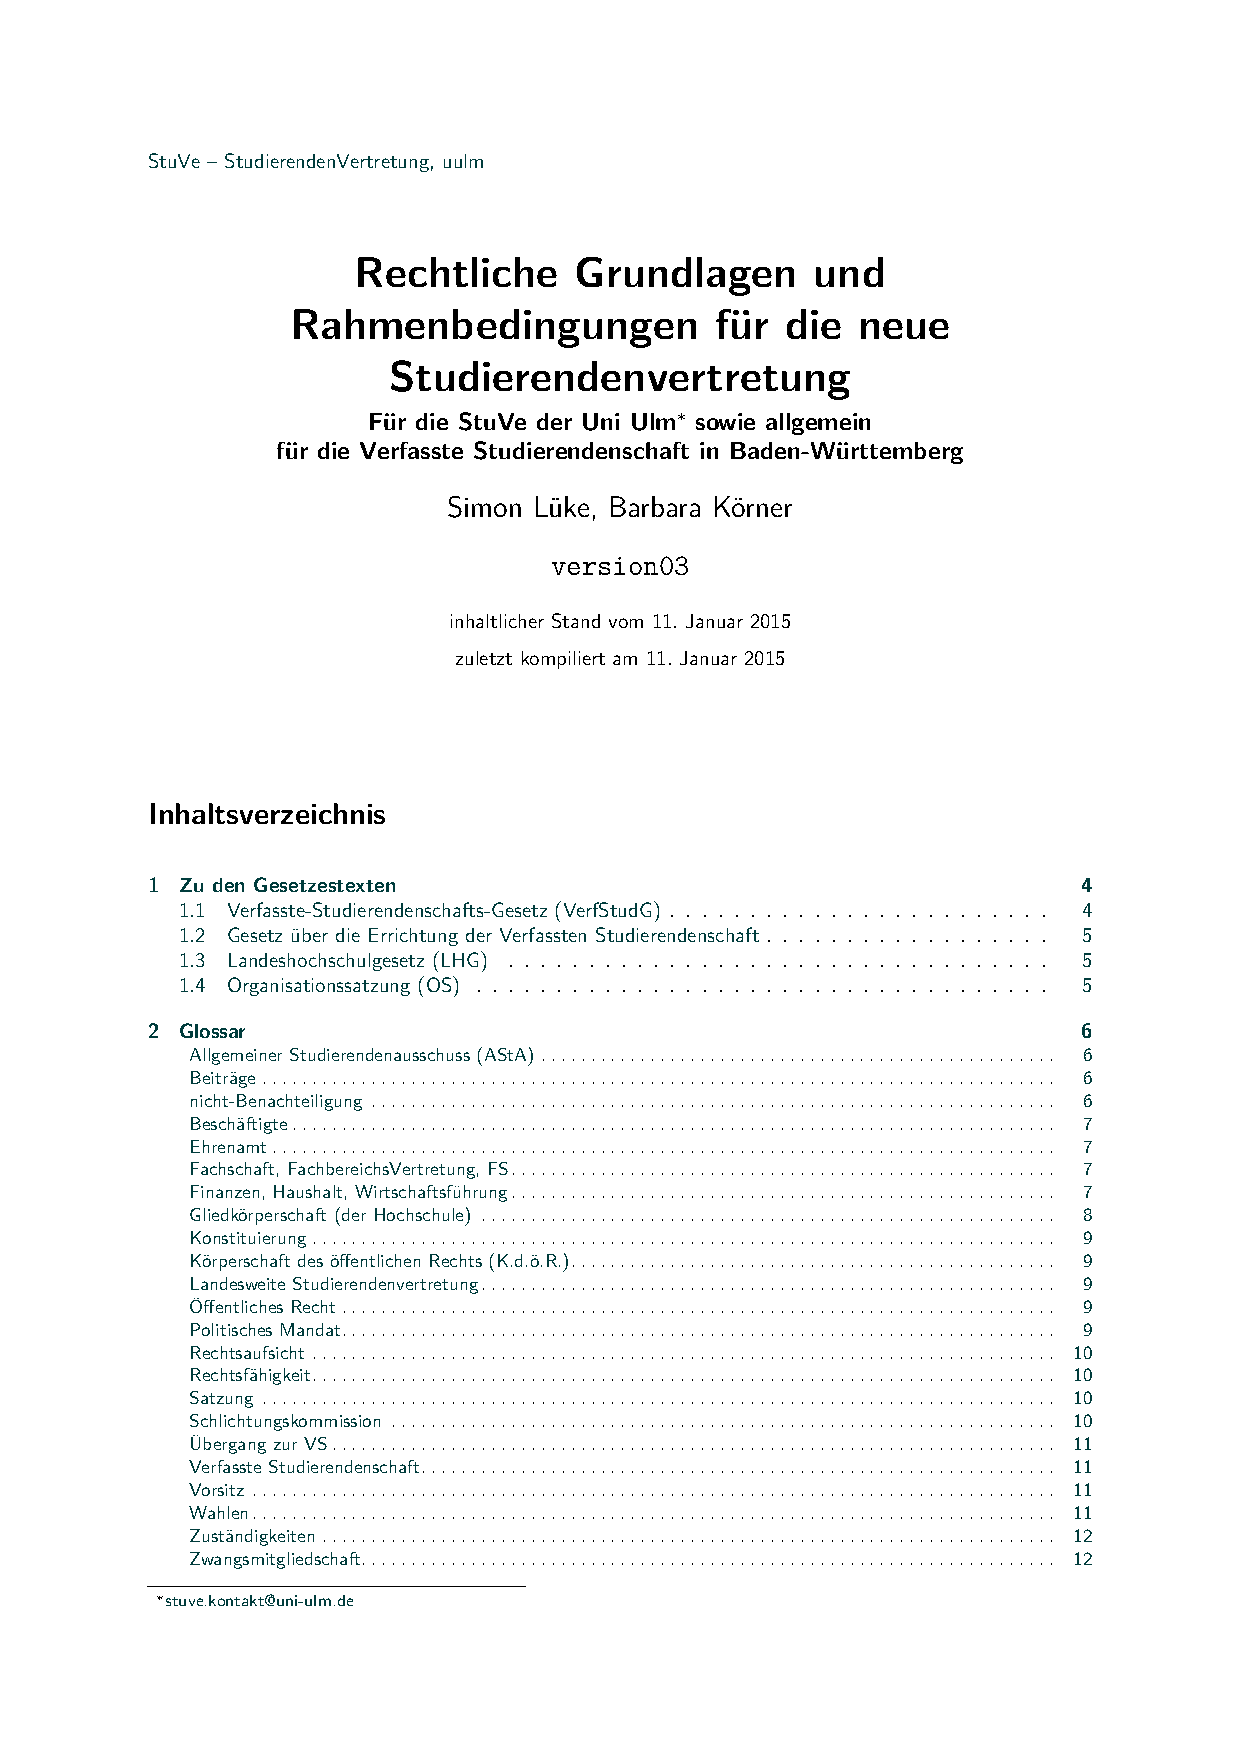
\includepdf
[
pages = 1-16,
trim = 2cm 2cm 2cm 1cm
]
{./teile/60-vs-dossier-rechtliche-rahmenbedingungen.pdf}



\chapter{Grafiken}

\clearpage

\addcontentsline{toc}{section}{Übersicht}

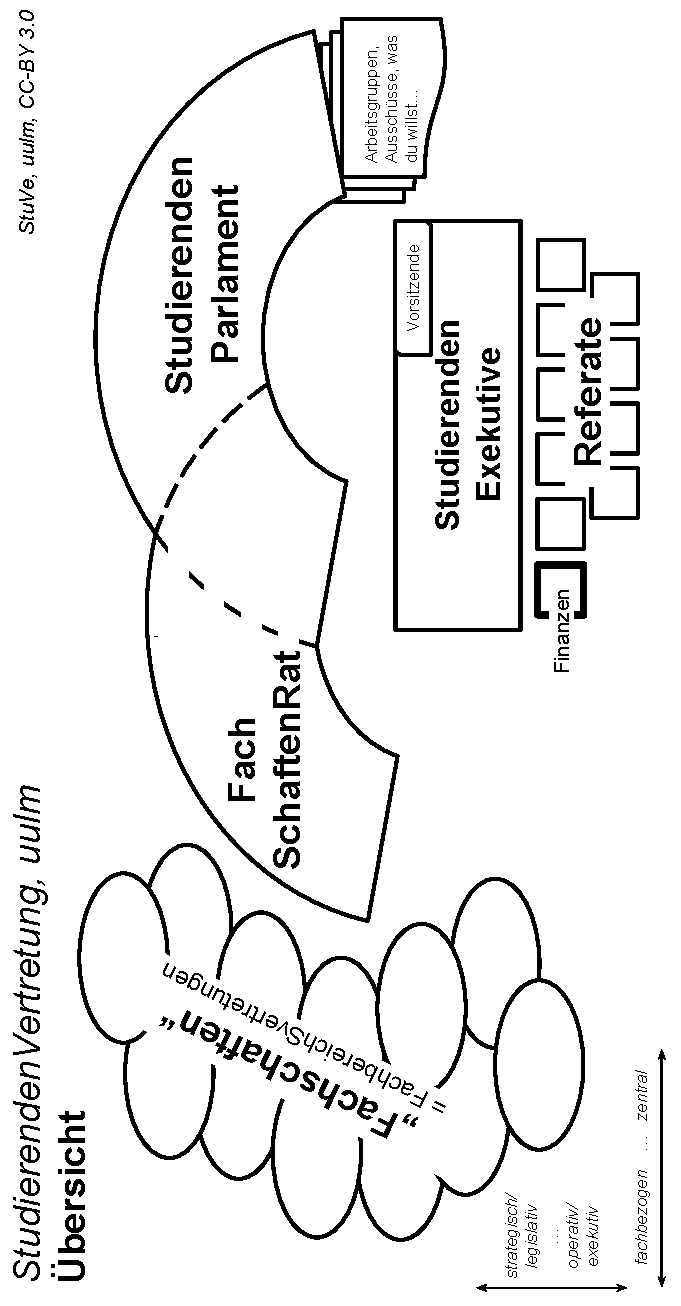
\includepdf
	[
		height = 0.9\paperheight,
		width = 0.8\paperwidth,
		keepaspectratio
	]
	{./teile/91-struktur-uebersicht.pdf}


\addcontentsline{toc}{section}{Studentische und akademische Selbstverwaltung}

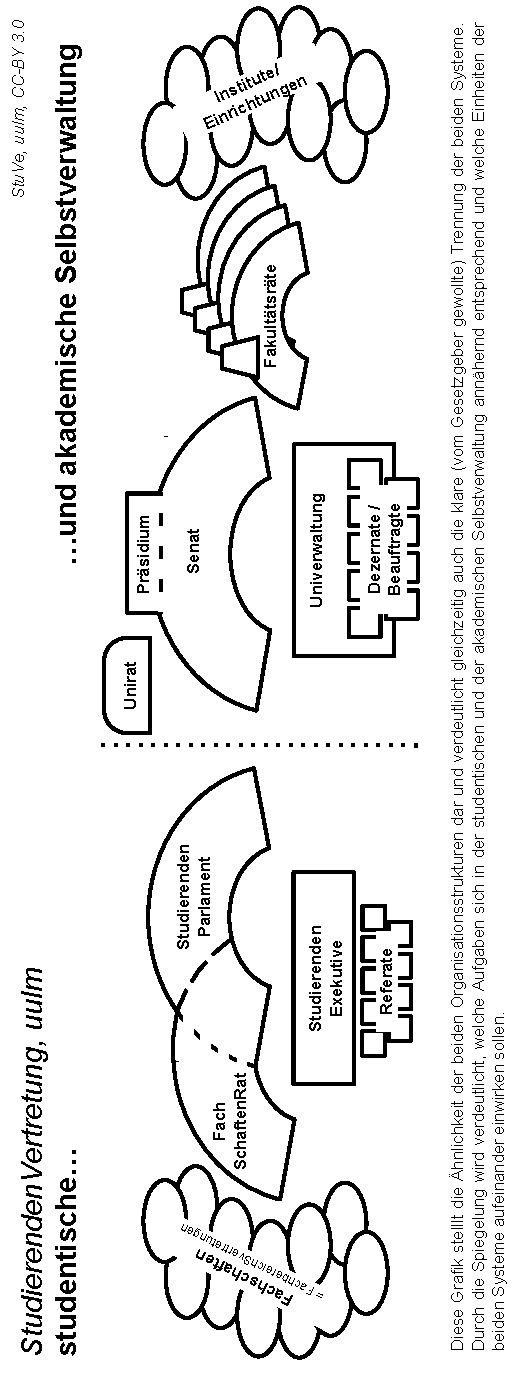
\includepdf
	[
		height = 0.9\paperheight,
		width = 0.8\paperwidth,
		keepaspectratio
	]
	{./teile/92-struktur-akad_selbstverw.pdf}


\addcontentsline{toc}{section}{Details: Besetzung, Interaktion und Kontrolle}

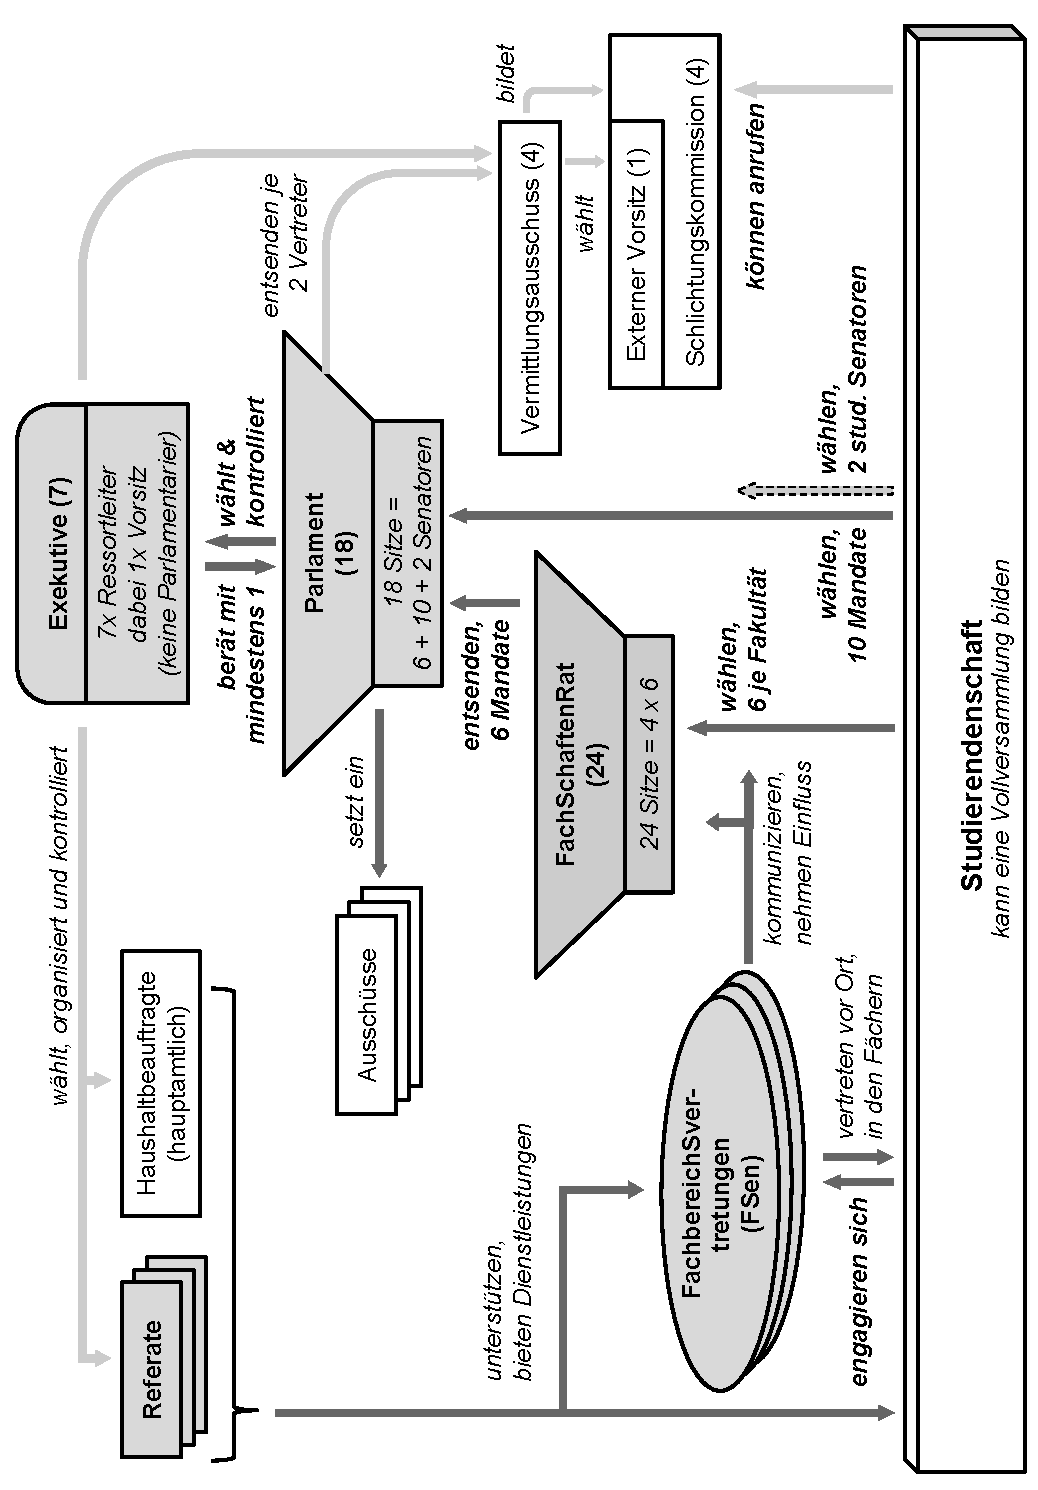
\includepdf
	[
		height = 0.9\paperheight,
		width = 0.8\paperwidth,
		keepaspectratio
	]
	{./teile/93-struktur-besetzung-kontrolle.pdf}



\backmatter

% !TeX root = ../stuve-handbuch-1.tex
% !TeX encoding = UTF-8
% !TeX spellcheck = de_DE
% !TeX program = pdflatex


\thispagestyle{empty}
\null\vfill
\begin{center}
	{\normalsize \textipa{/,ju:z3'bIlIti/}}
%	Freiraum!
\end{center}
\vfill\null\vfill
\clearpage

\thispagestyle{empty}
\null\vfill

\begin{center}
\begin{minipage}{0.7\textwidth}
%\scriptsize

Es gibt aktuell die folgenden \textbf{„StuVe-Handbücher“}

\textbf{\begin{enumerate}[\hspace{3em}1:]
	\item Gremien, Beschlüsse und Statuten
	\item Finanzen
	\item Veranstaltungsleitfaden
	\item Büro-ABC
\end{enumerate}}
\null

Alle sind im Wiki zu finden und dementsprechend gibt es dort immer den aktuellsten Stand: \url{https://wiki.asta.uni-ulm.de/asta/Handbuch}. Bisweilen wird – wie hier vorliegend – von manchen Handbüchern auch eine gedruckte Version erstellt.

\end{minipage}
\end{center}


\vfill\null\vfill
%\vspace{16.5cm}
\begin{center}
	
\includegraphics[keepaspectratio, width=5em]{./grafiken/stuve_logo_gedreht-leicht_grau.png}\\
	\textcolor{black!40}{\large \textbf{uuulm}}
\end{center}



\end{document}
